\section{Proposed method: the expected-cost hologram}\label{sec:proposed-method}

\subsection{Idea}

A hologram computed for the nominal system places each trap at an optimum of the nominal cost. The aberration then moves the traps off that optimum in directions the nominal cost does not see, and the intensities of the traps change by amounts that depend on how the hologram
phases are arranged, not only on how large the aberration is. Two holograms with the same nominal intensities can respond to the same wavefront error very differently, because the first-order response of each trap intensity to each aberration coefficient is a
property of the phase pattern. The idea is to choose, among the many holograms that equalize the traps at the nominal system, the one whose response to the aberrations of the prior is small, by minimizing the expected cost in Eq.~\eqref{eq:problem} instead of the cost at one point.
The method needs no wavefront measurement and no change of the optical train: it leaves the correction in place and designs for the residual. It starts from the hologram of phase-fixed WGS, which is already a minimizer of the nominal cost to a good approximation, so that the
expected-cost steps trade a small nominal spread and a small efficiency for a flatter response.

\subsection{Derivation}

\paragraph{Step 1, the expected cost.} Because the aberration is an additive phase, the cost at one aberration is the nominal cost at a shifted phase, $L(\phi,a)=L_0(\phi+\psi(a))$, where $L_0$ is the cost of Eq.~\eqref{eq:metrics} at no aberration. The expected cost is
$J(\phi)=\mathbb E_aL_0(\phi+\psi(a))$. Its value and gradient need the nominal cost and gradient at shifted phases only.

\paragraph{Step 2, what the expectation adds to the nominal cost.} For a small prior scale $s$, expand $L_0(\phi+\psi(a))$ to the second order in $a$ and take the expectation, with $\mathbb E a_k=0$ and $\mathbb E a_ka_l=s^2\delta_{kl}$:
\begin{equation}
J(\phi)=L_0(\phi)+\frac{s^2}{2}\sum_{k\in\mathcal K}\frac{\partial^2L_0(\phi+\psi(a))}{\partial a_k^2}\Big|_{a=0}+O(s^4).\label{eq:taylor}
\end{equation}
The second term is the curvature of the cost along each aberration mode. The chain rule, with $\partial\psi_j/\partial a_k=2\pi Z_k(x_j,y_j)$, gives $\partial^2L_0/\partial a_k^2=(2\pi)^2\,\mathbf z_k^{\!\top}\mathbf H(\phi)\,\mathbf z_k$ where $\mathbf z_k$ is the vector of the mode over the pixels and
$\mathbf H$ is the Hessian of $L_0$ in the pixel phases. A hologram with a small penalty sits where the cost is flat along the subspace spanned by the aberration modes.

\paragraph{Step 3, the structure of the curvature.} Write $G_{mk}=\partial I_m/\partial a_k$ for the first-order response of trap $m$ to mode $k$ at the nominal system. By the chain rule with $\partial\psi_j/\partial a_k=2\pi Z_k(x_j,y_j)$ and the derivative of $I_m$ in the pixel phase (Step 5), the response has the closed form
\begin{equation}
G_{mk}=-\frac{4\pi}{N^2}\sum_jA_jZ_k(x_j,y_j)\operatorname{Im}\Big[\bar V_m\,e^{i(\phi_j-\Delta_j^m)}\Big],\label{eq:response}
\end{equation}
a weighted sum over the pixels in which the mode enters as a weight and the phase of the hologram decides the sign: the same mode raises the intensity of one trap and lowers that of another according to the phases the hologram gives the pixels. Differentiating the cost of Eq.~\eqref{eq:metrics} twice gives
\begin{equation}
\frac{\partial^2L_0}{\partial a_k^2}=\frac{2}{\sum_nT_n^2}\Big[\sum_mG_{mk}^2+\sum_m(I_m-T_m)\frac{\partial^2I_m}{\partial a_k^2}\Big],\label{eq:gaussnewton}
\end{equation}
the sum of a Gauss--Newton term, which is non-negative and measures how strongly the intensities respond to the mode, and a residual term, which vanishes when the traps sit at their targets. The robust cost therefore contains the quantity $\sum_{m,k}G_{mk}^2$, the total
first-order intensity variance that the aberration prior induces (Section~\ref{sec:theory} shows that it bounds the expected squared spread).

\paragraph{Step 4, replacing the expectation.} A Monte Carlo average of $L_0$ over random draws of $a$ makes the cost noisy: two evaluations at the same $\phi$ differ, and a line search that needs a decrease between two points cannot decide. A deterministic set removes that noise. The $2K$
sigma points, a pair $\pm s\sqrt K$ on one mode at a time, have mean zero and covariance exactly $s^2I_K$:
\begin{equation}
\mathcal S=\big\{\pm s\sqrt K\,\mathbf e_k\ :\ k\in\mathcal K\big\},\qquad J_{\mathcal S}(\phi)=\frac1{2K}\sum_{\mathbf c\in\mathcal S}L_0\big(\phi+\psi(\mathbf c)\big).\label{eq:sigma}
\end{equation}
For $K=8$ and $s=\parAb$ waves the 16 points lie at $\pm\parAbSqrt$ waves on one mode, a point whose rms wavefront ($\parAbRms$ waves) equals that of the typical draw. Section~\ref{sec:theory} shows that $J_{\mathcal S}$ equals the Gaussian expectation through the second order in $s$. Figure~\ref{fig:design} places the points among the draws of the evaluation ensemble in the plane of two modes, and shows that the sixteen points share one rms wavefront, close to that of the typical draw.

\begin{figure}[t]
\centering
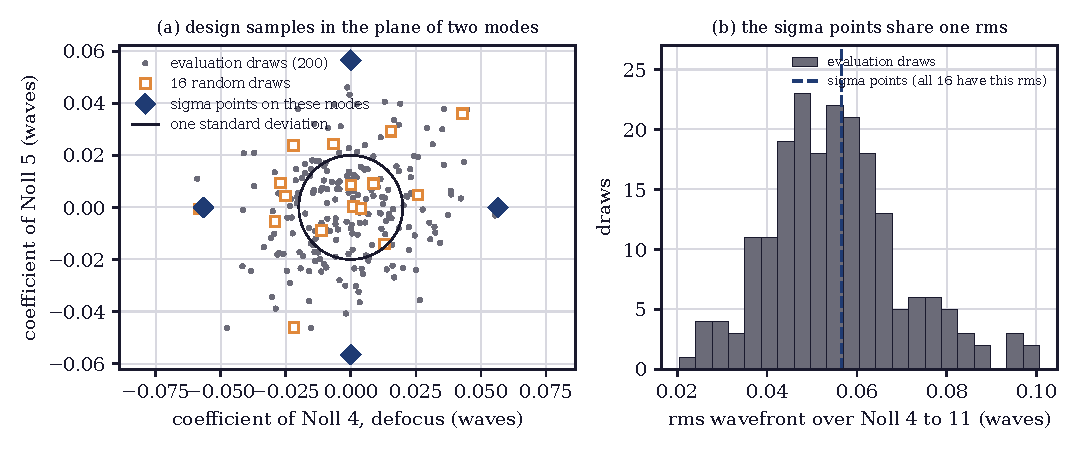
\includegraphics[width=\textwidth]{fig-design.pdf}
\caption{(a) Design samples in the plane of the coefficients of Noll modes 4 and 5: the four sigma points on these two modes, 16 random draws of the alternative design, and the 200 draws of the evaluation ensemble, with the circle of one standard deviation. (b) The rms wavefront over the eight modes of the 200 evaluation draws, and the common rms of the sigma points.}
\label{fig:design}
\end{figure}

\paragraph{Step 5, closed-form gradient.} From Eq.~\eqref{eq:forward}, $\partial I_m/\partial\phi_j=-\frac{2A_j}{N^2}\operatorname{Im}\big[\bar V_me^{i(\phi_j-\Delta_j^m)}\big]$, so for the nominal cost at a shifted phase $\phi'=\phi+\psi(\mathbf c)$,
\begin{equation}
\frac{\partial L_0}{\partial\phi_j}\Big|_{\phi'}=-\frac{4A_j}{N^2\sum_nT_n^2}\operatorname{Im}\Big[\sum_m\big(I_m(\phi')-T_m\big)\,\bar V_m(\phi')\,e^{i(\phi'_j-\Delta_j^m)}\Big],\qquad \nabla_\phi J_{\mathcal S}=\frac1{2K}\sum_{\mathbf c\in\mathcal S}\nabla_\phi L_0\big|_{\phi+\psi(\mathbf c)}.\label{eq:gradient}
\end{equation}
Since the aberration is a constant offset in the phase, the gradient of the expected cost with respect to the pixel phases is the average of the unperturbed gradients at the shifted phases, and each term is one forward and one adjoint evaluation of the point-trap model.

\paragraph{Step 6, the level and the solver.} The target of Eq.~\eqref{eq:metrics} is an absolute level: $T_m=\ell e_0w_m/\sum_nw_n$ with $e_0$ the efficiency of the starting hologram and $\ell=\parLevel$. The scale of the intensities is not refitted during the descent, so that the optimizer cannot lower the
expected cost by dimming all traps. A level below the efficiency of the start asks the hologram to give up a part of its nominal intensity; Section~\ref{sec:ablation} measures the trade-off in $\ell$, and Section~\ref{sec:results} shows that the level plays the role of the mean intensity that the aberrations remove. The cost $J_{\mathcal S}$ is smooth and deterministic, which is what the nonlinear conjugate gradient of Fletcher and
Reeves~\cite{fletcher1964} needs: with the gradient $\mathbf g_i$ at iterate $\phi_i$,
\begin{equation}
\mathbf d_i=-\mathbf g_i+\gamma_i\mathbf d_{i-1},\qquad \gamma_i=\frac{\|\mathbf g_i\|^2}{\|\mathbf g_{i-1}\|^2},\qquad \phi_{i+1}=\phi_i+\alpha_i\mathbf d_i,\label{eq:cg}
\end{equation}
with $\alpha_i$ from a strong-Wolfe line search (constants $c_1=10^{-4}$, $c_2=0.1$; $c_2<1/2$ keeps the directions descent directions)~\cite{nocedal2006}, and a restart from steepest descent when a direction fails.

\paragraph{Variant with random draws.} When the prior includes random displacements of the traps, the cost cannot be written as a function of the phase offset alone, and the product uses $Q$ random draws resampled at every step with Adam~\cite{kingma2015}:
\begin{equation}
\mathbf m_i=\beta_1\mathbf m_{i-1}+(1-\beta_1)\mathbf g_i,\quad \mathbf v_i=\beta_2\mathbf v_{i-1}+(1-\beta_2)\mathbf g_i^2,\quad \phi_{i+1}=\phi_i-\mathrm{lr}\,\frac{\mathbf m_i/(1-\beta_1^i)}{\sqrt{\mathbf v_i/(1-\beta_2^i)}+\epsilon}.\label{eq:adam}
\end{equation}
This design is automatic when a pointing prior is set; it is the design measured in Section~\ref{sec:results} for pointing errors.

\subsection{Design choices}

Four choices shape the method, and each has an alternative that the experiments or the theory discard or leave open. The start is the hologram of phase-fixed WGS and not a random phase or the output of a nominal conjugate-gradient run: the start is already a good minimizer of the nominal cost, it is the baseline of the comparison, and so the expected-cost steps are the only difference between the baseline and the result. A random start would
conflate the benefit of the expected cost with the benefit of reaching a good nominal hologram at all, which some of the published methods of Table~\ref{tab:pub} do not reach at the budgets of the comparison.

The expectation is taken by sigma points and not by random draws because the line search of the solver compares the cost at two points along a direction, and a cost that changes between evaluations at the same point gives no reliable decrease. Random draws held fixed during the descent remove the noise but then optimize for those draws only, and resampled draws need a stochastic optimizer with its smaller steps; the measurements of the ablation put the sigma points ahead of fixed random draws of the same number and of twice the number.

The target level $\ell$ is an absolute intensity that is not rescaled during the descent. If the scale were refitted at each evaluation (the least-squares scale of the cost of Polin et al.~\cite{polin2005}, which the engine offers), the optimizer could lower the expected cost by dimming the traps uniformly; fixing the level at a fraction of the start efficiency prevents it, and gives the user the dial between efficiency and robustness that Section~\ref{sec:ablation} measures. The cost is the sum of squared intensity errors; the same code accepts any even power, and the square is the one that the closed forms of Section~\ref{sec:theory} use.

The designed modes are Noll 4 to 11 and not a larger set because piston changes no intensity and the two tilts move the whole pattern (they belong to the alignment, not to the residual), because Noll 4 to 11 are the modes that the sensorless correction of the product searches and that its acceptance set injects, and because the number of sigma points grows with the number of modes: $2K$ evaluations per cost. A larger set would add points, not change the algorithm, and the ablation shows that a design that does not cover the modes of the ensemble does not protect against them.

\subsection{Algorithm}

Algorithm~\ref{alg:robust} is the aberration design measured in the main experiment, and Algorithm~\ref{alg:sample} the variant with random draws and Adam. The first calls the phase-fixed WGS routine of the product with its documented parameters ($n_{\mathrm{fix}}=12$ weighted iterations before the focal phases are frozen) and then
takes conjugate-gradient steps on the sigma-point cost. Both algorithms return the phase wrapped to $[0,2\pi)$. The descent itself runs on the unwrapped phase, since the field depends on the phase through its exponential and the gradient is a smooth function of it; the wrap at the end changes no intensity. In Algorithm~\ref{alg:robust} the aberration phases of the sixteen points are computed once, because they do not depend on the hologram, so the inner loop is only the forward and adjoint evaluations of the point-trap model. In Algorithm~\ref{alg:sample} the draws change at every step, the traps move with the displacement draw, and the cost is therefore evaluated on a different system at each of the $Q$ draws; its value is a noisy estimate of the expected cost, which is why the algorithm uses a stochastic optimizer and no line search.

\begin{algorithm}[t]
\caption{Aberration-robust hologram with the sigma-point design (the design of the main experiment).}
\label{alg:robust}
\begin{algorithmic}[1]
\Require traps $\{(x_m,y_m,w_m)\}$, prior scale $s$, designed modes $\mathcal K$, level $\ell$, WGS iterations $n_0$, CG iterations $n$, seed
\State $\phi_0\gets$ phase-fixed WGS for $n_0$ iterations from the random-superposition start of the seed
\State $e_0\gets\sum_m|V_m(\phi_0)|^2$; $\ T_m\gets\ell e_0w_m/\sum_nw_n$
\State $\mathcal S\gets\{\pm s\sqrt{|\mathcal K|}\,\mathbf e_k:k\in\mathcal K\}$; precompute $\psi(\mathbf c)$ for every $\mathbf c\in\mathcal S$
\For{$i=1,\dots,n$}
\State $J\gets0$; $\ \mathbf g\gets\mathbf 0$
\For{each $\mathbf c\in\mathcal S$}
\State evaluate $V_m$ at $\phi_{i-1}+\psi(\mathbf c)$ (forward); $L_0$ from Eq.~\eqref{eq:metrics}; $\nabla L_0$ from Eq.~\eqref{eq:gradient} (adjoint)
\State $J\gets J+L_0/|\mathcal S|$; $\ \mathbf g\gets\mathbf g+\nabla L_0/|\mathcal S|$
\EndFor
\State $\mathbf d\gets-\mathbf g+\gamma\mathbf d_{\mathrm{prev}}$ (Eq.~\eqref{eq:cg}); restart with $\mathbf d\gets-\mathbf g$ if $\mathbf g^{\top}\mathbf d\ge0$
\State find $\alpha$ by the strong-Wolfe search (each trial repeats the inner loop); $\ \phi_i\gets\phi_{i-1}+\alpha\mathbf d$
\EndFor
\State \Return $\phi_n\bmod2\pi$
\end{algorithmic}
\end{algorithm}

\begin{algorithm}[t]
\caption{Variant with random draws, Adam and a pointing prior.}
\label{alg:sample}
\begin{algorithmic}[1]
\Require as Algorithm~\ref{alg:robust}, plus the pointing scale $s_p$ in focal bins, draws per step $Q$, rate $\mathrm{lr}$
\State $\phi_0$, $e_0$, $T_m$ as in Algorithm~\ref{alg:robust}; $\mathbf m,\mathbf v\gets\mathbf 0$
\For{$i=1,\dots,n$}
\For{$q=1,\dots,Q$}
\State draw $a\sim\mathcal N(0,s^2I_K)$ and displacements $d^x_m,d^y_m\sim\mathcal N(0,s_p^2)$ bins for every trap
\State evaluate $L_0$ and $\nabla L_0$ at $\phi_{i-1}+\psi(a)$ for the traps moved by $(d^x_m,d^y_m)$; average over $q$
\EndFor
\State update $\mathbf m,\mathbf v$ and $\phi_i$ by Eq.~\eqref{eq:adam}
\EndFor
\State \Return $\phi_n\bmod2\pi$
\end{algorithmic}
\end{algorithm}

\subsection{Parameters}

Table~\ref{tab:params} lists every parameter with its value in the experiments and where the value comes from. The values are those of the implementation; the design amplitude $s$ is a choice of the product that the paper states and measures (Sections~\ref{sec:ablation} and~\ref{sec:results}), not a figure
taken from a published instrument, and the number of random draws per step ($Q=\parQ$) follows the range of 8 to 32 samples per iteration recorded in the research that preceded the implementation. Two of the parameters carry most of the behaviour and are therefore varied in the ablation: the design amplitude $s$, which sets how far the sigma points sit from the nominal system, and the level $\ell$, which sets how much room the hologram has to move without paying nominal error. The others are conventions of the solver (the Wolfe constants are the textbook ones and the Adam constants are those of its authors) or of the start (the 30 iterations of phase-fixed WGS are the iteration count at which the baseline of the comparison is scored).

\begin{table}[t]
\centering\small
\caption{Parameters of the aberration-robust hologram: the value used in the experiments and its origin. The values are read from the implementation by the measurement script.}
\label{tab:params}
\begin{tabular}{@{}p{3.1cm} p{2.4cm} p{8.6cm}@{}}
\toprule
Parameter & Value & Origin\\
\midrule
Design amplitude $s$ & \parAb{} waves per mode & stated choice of the product; ensemble rms \parAbRms{} waves, Strehl about 0.88\\
Designed modes $\mathcal K$ & Noll 4 to 11 & defocus, astigmatisms, comas, trefoils and spherical; piston and tilts excluded\\
Sigma points & 16 & $\pm s\sqrt8$ on one mode at a time\\
Target level $\ell$ & \parLevel & trade-off measured in Section~\ref{sec:ablation}\\
Start & phase-fixed WGS, \parWarm{} iterations & the baseline method, with $n_{\mathrm{fix}}=12$ weighted iterations before the phase is frozen\\
CG iterations $n$ & \parIters{} & budget of the acceptance test\\
Line search & strong Wolfe & $c_1=10^{-4}$, $c_2=0.1$, cubic interpolation; first trial moves the largest pixel by 0.1 rad\\
Draws per step $Q$ & \parQ{} & range of 8 to 32 per iteration of the research record\\
Adam rate & \parLr{} & $\beta_1=0.9$, $\beta_2=0.999$, $\epsilon=10^{-8}$\\
\bottomrule
\end{tabular}
\end{table}

\subsection{Complexity}

One evaluation of the cost and gradient at one sigma point costs a forward and an adjoint evaluation of the point-trap model, each a product of $N\times N$ and $N\times M$ matrices in the separable form, $O(N^2M)$ operations. One conjugate-gradient iteration evaluates the $2K=16$ sigma points once per trial step of
the line search, so the cost of a run is $O\big(n\,t_{\mathrm{ls}}\,2K\,N^2M\big)$ with $t_{\mathrm{ls}}$ the number of trial steps per iteration, against $O(n\,t_{\mathrm{ls}}N^2M)$ for conjugate gradient on the nominal cost, a factor $2K$ more. The ensemble evaluation of the result is $200$ forward evaluations per hologram.
In the experiments ($N=256$, $M=100$, $n=\parIters$) one run of the robust hologram took a median of \runSeconds{} seconds of wall-clock time per seed with \workersUsed{} processes sharing the machine, so the figure is an upper bound of an unloaded run. The cost of a run is linear in the number of sigma points, and so in the number of designed modes. The method is a design computed once per array, offline,
and is not a method for the live loop of a rearrangement.

\subsection{Implementation}

The method is implemented in the repository of the product as the module \texttt{pipeline.model.holo.methods.beyond.b4\_robust}, which exposes the run function with the parameters of Table~\ref{tab:params}, the sigma-point generator and an ensemble evaluator that returns the efficiency, the 95th percentile and the sorted spreads
over a seeded ensemble. It builds on the cost class and the conjugate-gradient and Adam routines of the shared optimization module and on the phase-fixed WGS of the weighted-GS family, so that its start is the published method itself and not a copy of its equations. All randomness comes from a portable
generator (xoshiro128** seeded by SplitMix32) so that a seed gives the same hologram on every machine. The experiments of this paper call the module through its public functions and, for the ablation, a replica of the sigma-point loop that takes the design samples as an argument; the replica reproduces the module's hologram on the default
configuration to \replicaDiff{} rad in the largest pixel phase.
